\subsection[gcc]{The Compiling Chain}

\begin{frame}[fragile]
  \frametitlecpp[17]{The compiling chain}
  \center
  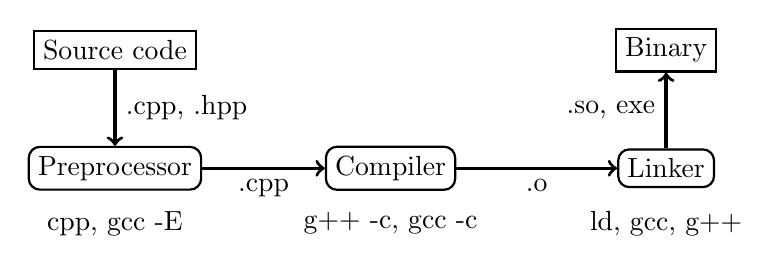
\begin{tikzpicture}
    \draw[thick] node (code) at(0,0) [rectangle,draw] {Source code}
                 node (cpp) at(0, -1.5cm) [rectangle,rounded corners,draw] {Preprocessor}
                 node (gcc) at(3.5cm,-1.5cm) [rectangle,rounded corners,draw] {Compiler}
                 node (ld) at(7cm,-1.5cm) [rectangle,rounded corners,draw] {Linker}
                 node (bin) at(7cm,0) [rectangle,draw] {Binary}
                 node at(0, -2.2cm) {cpp, gcc -E}
                 node at(3.5cm, -2.2cm) {g++ -c, gcc -c}
                 node at(7cm, -2.2cm) {ld, gcc, g++};
    \draw[very thick,->] (code) -- (cpp) node [midway,right] {.cpp, .hpp};
    \draw[very thick,->] (cpp) -- (gcc) node [midway,below] {.cpp};
    \draw[very thick,->] (gcc) -- (ld) node [midway,below] {.o};
    \draw[very thick,->] (ld) -- (bin) node [midway,left] {.so, exe};
  \end{tikzpicture}
  \begin{block}{The steps}
    \begin{description}
    \item[cpp]
        the preprocessor \\
        handles the \# directives (macros, includes) \\
        creates ``complete'' source code (ie. translation unit)
    \item[g++]
        the compiler \\
        creates machine code from \cpp code
    \item[ld]
        the linker \\
        links several binary files into libraries and executables
    \end{description}
  \end{block}
\end{frame}

\begin{frame}[fragile]
  \frametitle{Compilers}
  \begin{block}{Available tools}
    \begin{description}
    \item[\href{http://gcc.gnu.org/}{\beamergotobutton{gcc}}]
        the most common and most used\\
        free and open source
    \item[\href{http://clang.llvm.org/}{\beamergotobutton{clang}}]
        drop-in replacement of gcc \\
        slightly better error reporting \\
        free and open source, based on LLVM
    \item[\href{https://www.intel.com/content/www/us/en/developer/tools/oneapi/dpc-compiler.html\#gs.dyllp0}{\beamergotobutton{icc} \beamergotobutton{icx}}]
        Intel's compilers, proprietary but now free \\
        optimized for Intel hardware \\
        icc being replaced by icx, based on LLVM
    \item[\href{https://visualstudio.microsoft.com/}{\beamergotobutton{Visual \cpp / MSVC}}]
      Microsoft's C++ compiler on Windows
    \end{description}
  \end{block}
  \begin{alertblock}{My preferred choice today}
    \begin{itemize}
      \item \alert{gcc} as the de facto standard in HEP
      \item \hspace{0pt}\alert{clang} in parallel to catch more bugs
    \end{itemize}
  \end{alertblock}
\end{frame}

\begin{frame}[fragile]
  \frametitle{Useful compiler options (gcc/clang)}
  \begin{block}{Get more warnings}
    \begin{description}
      \item[-Wall -Wextra] get all warnings
      \item[-Werror] force yourself to look at warnings
    \end{description}
  \end{block}
  \begin{block}{Optimization}
    \begin{description}
      \item[-g] add debug symbols
      \item[-Ox] 0 = no opt., 1-2 = opt., 3 = highly opt. (maybe larger binary), g = opt. for debugging
    \end{description}
  \end{block}
  \begin{block}{Compilation environment}
    \begin{description}
      \item[\texttt{-I} \textless{}path\textgreater] where to find header files
      \item[\texttt{-L} \textless{}path\textgreater] where to find libraries
      \item[\texttt{-l} \textless{}name\textgreater] link with libname.so
      \item[\texttt{-E / -c}] stop after preprocessing / compilation
    \end{description}
  \end{block}
\end{frame}

\begin{frame}[fragile]
  \frametitle{Makefiles}
  \begin{block}{Why to use them}
    \begin{itemize}
    \item an organized way of describing building steps
    \item avoids a lot of typing
    \end{itemize}
  \end{block}
  \begin{block}{Several implementations}
    \begin{itemize}
    \item raw Makefiles: suitable for small projects
    \item cmake: portable, the current best choice
    \item automake: GNU project solution
    \end{itemize}
  \end{block}
  \begin{minted}{makefile}
    test : test.cpp libpoly.so
        $(CXX) -Wall -Wextra -o $@ $^
    libpoly.so: Polygons.cpp
        $(CXX) -Wall -Wextra -shared -fPIC -o $@ $^
    clean:
        rm -f *o *so *~ test test.sol
  \end{minted}
\end{frame}

\begin{frame}[fragile]
  \frametitle{CMake}
  \begin{block}{}
    \begin{itemize}
      \item a cross-platform meta build system
      \item generates platform-specific build systems
      \item see also this \href{https://www.youtube.com/watch?v=eC9-iRN2b04}{basic} and \href{https://www.youtube.com/watch?v=bsXLMQ6WgIk}{detailed} talks
    \end{itemize}
  \end{block}
  \begin{block}{Example CMakeLists.txt}
    \begin{minted}[linenos=true,autogobble]{cmake}
      cmake_minimum_required(VERSION 3.18)
      project(hello CXX)

      find_package(ZLIB REQUIRED) # for external libs

      add_executable(hello main.cpp util.h util.cpp)
      target_compile_features(hello PUBLIC cxx_std_17)
      target_link_libraries(hello PUBLIC ZLIB::ZLIB)
    \end{minted}
  \end{block}
\end{frame}

\begin{frame}[fragile]
  \frametitle{CMake - Building}
  \begin{block}{Building a CMake-based project}
    Start in the directory with the top-level \texttt{CMakeLists.txt}:
    \begin{minted}[linenos=true,autogobble]{bash}
      mkdir build # will contain all build-related files
      cd build
      cmake ..    # configures and generates a build system
      cmake -DCMAKE_BUILD_TYPE=Release .. # pass arguments
      ccmake .    # change configuration using terminal GUI
      cmake-gui . # change configuration using Qt GUI
      cmake --build . -j8    # build project with 8 jobs
      cmake --build . --target hello  # build only hello
      sudo cmake --install . # install project into system
      cd ..
      rm -r build # clean everything
    \end{minted}
  \end{block}
\end{frame}

\begin{frame}[fragile]
  \frametitle{Compiler chain}
  \begin{exercise}{Compiler chain}
    \begin{itemize}
    \item go to code/functions
    \item preprocess functions.cpp (cpp or gcc -E -o output)
    \item compile functions.o and Structs.o (g++ -c -o output)
    \item use nm to check symbols in .o files
    \item look at the Makefile
    \item try make clean; make
    \item see linking stage of the final program using g++ -v
      \begin{itemize}
      \item just add a -v in the Makefile command for functions target
      \item run make clean; make
      \item look at the collect 2 line, from the end up to ``-o functions''
      \end{itemize}
    \item see library dependencies with `ldd functions`
    \end{itemize}
  \end{exercise}
\end{frame}
